\section{X-ray diffraction}
One way where the 'Von Laue-Bragg' condition can be observed is in x-ray diffraction. The 'Von Laue-Bragg' condition states that an inciding electron is or scattered or stays unscattered when colliding with a crystal. This scattering is elastic thus the amplitude of the wave function does not change. This is illustrated in figure \ref{fig:vonlaue}.
\begin{figure}[b]
    \centering
    \begin{tikzpicture}
        \draw[->, black]	node[left] {$e^-$}(0, 0) to node[above]{incident} node[below]{$\vec{k}$} (2, 0);

        \draw[black] plot [smooth cycle] coordinates {(2.6, 0) (3.2, 0.6) (2.9, 0.7) (3.5, 1) (4.2, 0.9) (4.5, -0.3) (3.9, -0.2) (3.5, -0.7)} node [above=5mm, size=1pt]{CRYSTAL};

        \draw[->, black]	(5, 0.2) to node[above]{$\vec{k}'$}(6, 0.8) node[right=1mm]{$e^-$ (scattered)};
		\draw[->, black]	(5, 0) to node[below]{$\vec{k}$}(6, 0) node[right=1mm]{$e^-$ (unscattered)};
    \end{tikzpicture}
    \caption{X-ray diffraction on a lattice}
    \label{fig:vonlaue}
\end{figure}
Becuase the scattering is elastic we can state the following, define the wave as $e^{i\vec{k}\cdot\vec{r}}$:
\begin{align}
	E(\vec{k}) &= \frac{\hbar^2k^2}{2m}\\
	&= E(\vec{k}')\\
	&= \frac{\hbar^2k'^2}{2m}\\
	&\Rightarrow \abs{\vec{k}} = \abs{\vec{k}'}
\end{align}
One way of figuring out if an electron is scattered is to use the Fermi golden rule.

\section{Fermi golden rule}
\dfn{The fermi golden rule}{The fermi golden rule states that ($\tau_{\vec{k} \rightarrow \vec{k}'}$ is the mean time to have a diffraction):
\begin{equation}
	\frac{1}{\tau_{\vec{k} \rightarrow \vec{k}'}} = \frac{2\pi}{\hbar}\abs{<\vec{k}|V(\vec{r})|\vec{k}'>}^2\delta(E(\vec{k}) - E(\vec{k}'))
\end{equation}
}
We will look a bit further into this equation. We know that $V(\vec{r})=$ a periodic potential field of the crystal. Then
\begin{align}
	<\vec{k}|V(\vec{r})|\vec{k}'> \quad &= \int_{V}^{}d\vec{r}\frac{1}{\sqrt{V}}e^{i\vec{k}\cdot\vec{r}}V(\vec{r})\frac{1}{\sqrt{V}}e^{-i\vec{k}\cdot\vec{r}} \label{eqn:constants}\\
	&= \frac{1}{V}\sum_{\vec{R}}^{}\int_{\text{unit cell}}^{}d\vec{r}V(\vec{r}+\vec{R})e^{i(\vec{k}-\vec{k}')\cdot(\vec{r}+\vec{R})} \label{eqn:periodicity}
\end{align}
Equation \ref{eqn:constants} has normalization constants $\frac{1}{\sqrt{V}}$. Furthermore, in equation \ref{eqn:periodicity} we exploit hte periodicity of $V(\vec{r})$ and translation symmetry (section \ref{sec:trans_symm}). When is this integral in equation \ref{eqn:periodicity} non-zero?
\begin{equation}
	\text{The integral is non-zero } \iff \vec{k} - \vec{k}' = \vec{G} \text{ (the reciprocal lattice vector)} \label{eqn:Bragg_condition}
\end{equation}
By symmetry, we can leave $\vec{R}$ out of equation \ref{eqn:periodicity}, we get:
\begin{align}
	<\vec{k}|V(\vec{r})|\vec{k}'> \quad &= \frac{1}{V}\sum_{\vec{R}}^{}\int_{\text{unit cell}}^{}d\vec{r}V(\vec{r}+\vec{R})e^{i(\vec{k}-\vec{k}')\cdot\vec{r}}\\
	&\qquad\text{where } \int_{\text{unit cell}}^{}d\vec{r}V(\vec{r}+\vec{R})e^{i\vec{G}\cdot\vec{r}} = \tilde{V}(\vec{G})\\
	&\qquad\text{with } V(\vec{r}) = \sum_{\vec{G}}^{}\tilde{V}(\vec{G})e^{i\vec{G}\cdot\vec{r}}\\
	\iff & e^{i\vec{G}\cdot\vec{r}} = 1
\end{align}
As we know from section \ref{sec:reciproc_space} if $\vec{G} (= \vec{k} - \vec{k}')$ is not a reciprocal lattice vector, $\tilde{V}(\vec{G}) = 0$. $\vec{G}$ must be a lattice vector. The condition \ref{eqn:Bragg_condition} is the von Laue condition for constructive scattering.\par
So if we have elastic scattering, than the wavevectors and wavelengths are the same:
\begin{align}
	\abs{\vec{k}} &= \abs{\vec{k}'} \\
	\frac{2\pi}{\lamba} &= \frac{2\pi}{\lambda'}\\
	\iff \lambda &= \lambda'
\end{align}
If we have the same wavelength, this scattering introduces extra distance for different incoming waves, we can see that in figure \ref{fig:extradistance}
\begin{figure}
	\centering
	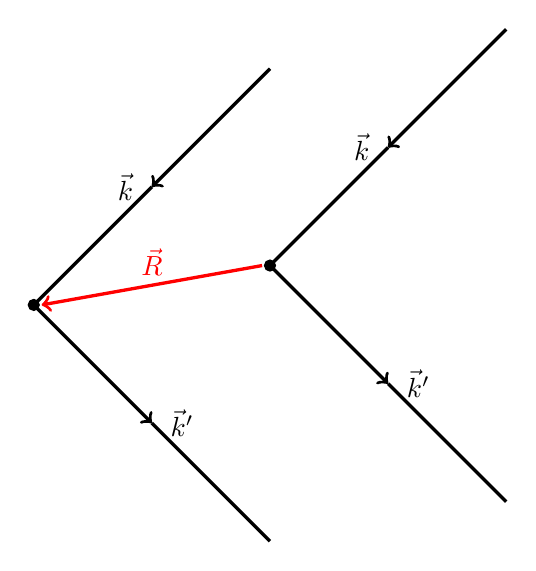
\begin{tikzpicture}
		\draw[->, black, very thick]	(3, 3) to (1.5, 1.5) node[left=1mm]{$\vec{k}$};
		\draw[-, black, very thick]		(1.5, 1.5) to (0, 0);

		\draw[->, black, very thick]	(6, 3.5) to (4.5, 2) node[left=1mm]{$\vec{k}$};
		\draw[-, black, very thick]		(4.5, 2) to (3, 0.5);

		\filldraw[black]	(0, 0) circle (2pt)
							(3, 0.5) circle (2pt);

		\draw[->, black, very thick]	(0, 0) to (1.5, -1.5) node[right=1mm]{$\vec{k}'$};
		\draw[-, black, very thick]		(1.5, -1.5) to (3, -3);

		\draw[->, black, very thick]	(3, 0.5) to (4.5, -1) node[right=1mm]{$\vec{k}'$};
		\draw[-, black, very thick]		(4.5, -1) to (6, -2.5);

		\draw[->, red, very thick] 	(2.9, 0.5) to (0.1, 0);
		\draw[red]		(1.5, 0.25) node[above]{$\vec{R}$};
	\end{tikzpicture}
	\caption{Extra distance for different wavevectors}
	\label{fig:extradistance}
\end{figure}
\subsection{Von Laue-Bragg condition} \label{sec:bragg}
abc

\section{Von Laue-Bragg condition}
abc

\section{The Brillouin Zone (BZ)} \label{sec:Brillouin}
abc
